\chapter{สถาปัตยกรรมฮาร์ดแวร์ระบบแปลงปลูกอัจฉริยะ}
\label{chap:hardware}

ระบบเกษตรกรรมแม่นยำสูง (Precision Agriculture) จำเป็นต้องอาศัยการตรวจวัดสภาวะแวดล้อมที่ครอบคลุมทั้ง 3 มิติหลัก ได้แก่ บรรยากาศรอบทรงพุ่ม (Microclimate) พลังงานรังสีแสงอาทิตย์ (Solar Radiation) และคุณสมบัติทางกายภาพเคมีในเขตรากพืช (Edaphic Zone) บทนี้นำเสนอการออกแบบสถาปัตยกรรมฮาร์ดแวร์ของระบบ \textbf{JC -AgriTech + AI}\index{JC-AgriTech} โดยประยุกต์ใช้ไมโครคอนโทรลเลอร์สมรรถนะสูงตระกูล ESP32-S3 บนบอร์ด ATD3.5-S3\index{ATD3.5-S3} ร่วมกับบอร์ดขยายสัญญาณ ATD3.5-S3 Farm1 Shield\index{Farm1 Shield}

\section{ภาพรวมสถาปัตยกรรมบอร์ดควบคุมและบอร์ดขยายสัญญาณ}

บอร์ดควบคุมหลักของระบบคือ \textbf{ATD3.5-S3} ซึ่งขับเคลื่อนด้วยชิปประมวลผล Dual-core Xtensa LX7 ความเร็วสัญญาณนาฬิกา 240 MHz มีหน่วยความจำ SRAM ขนาด 320 KB และ Flash Memory ขนาด 8 MB ในโหมด Dual I/O (DIO) พร้อมหน้าจอแสดงผลสีแบบสัมผัสชนิด IPS ขนาด 3.5 นิ้ว ความละเอียด $480 \times 320$ พิกเซล ควบคุมด้วยไอซีขับจอ ST7796 ผ่านการเชื่อมต่อแบบ SPI ความเร็วสูง\index{ST7796}

การเชื่อมต่อเซนเซอร์ภาคสนามกระทำผ่านบอร์ดขยายสัญญาณ \textbf{ATD3.5-S3 Farm1 Shield} ซึ่งเสียบประกบเข้ากับบอร์ดหลักโดยตรง ช่วยลดความซับซ้อนของการเดินสายสัญญาณและเพิ่มความคงทนต่อสภาพแวดล้อมในโรงเรือน โดยบอร์ดขยายสัญญาณประกอบด้วยจุดเชื่อมต่อมาตรฐาน 3 กลุ่มหลัก ได้แก่ ขั้วต่อสัญญาณดิจิทัล I2C ขั้วต่อสัญญาณแอนะล็อกสำหรับวัดความชื้นในดิน และขั้วต่อการสื่อสารเชิงอุตสาหกรรม RS485\index{RS485} พร้อมภาคจ่ายไฟเลี้ยง 12 V สำหรับโพรบวัดดินลึก

\begin{figure}[htbp]
    \centering
    \begin{minipage}[b]{0.48\textwidth}
        \centering
        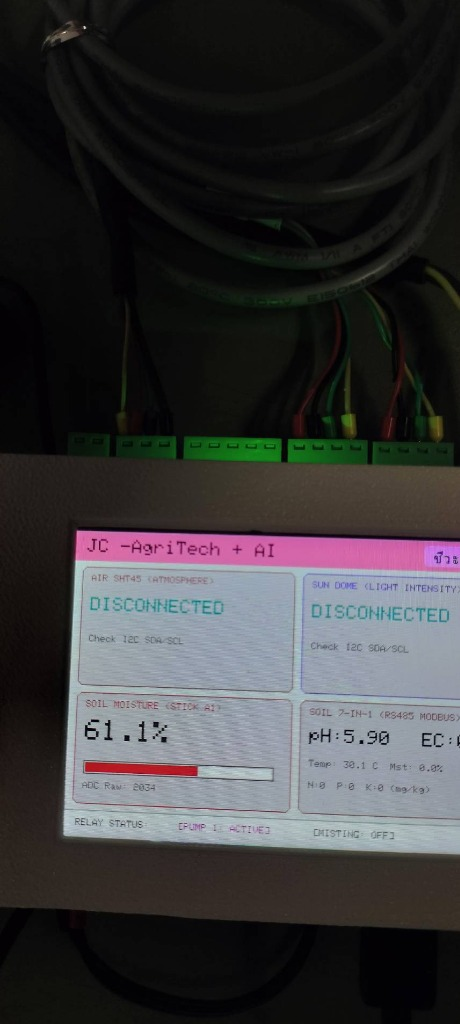
\includegraphics[height=5.0cm,width=\textwidth,keepaspectratio]{figures/board_overview.jpg}
        \caption{บอร์ดควบคุมหลัก ATD3.5-S3 พร้อมจอภาพ IPS}
        \label{fig:board_overview}
    \end{minipage}
    \hfill
    \begin{minipage}[b]{0.48\textwidth}
        \centering
        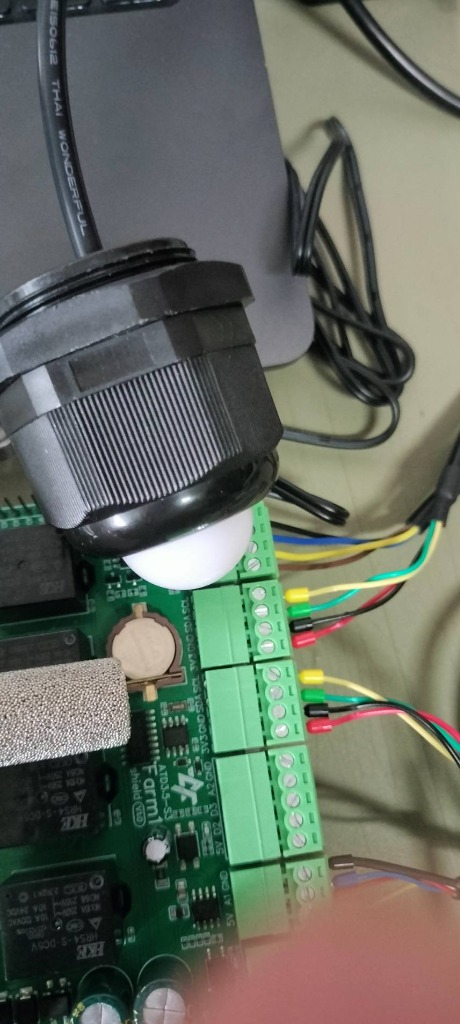
\includegraphics[height=5.0cm,width=\textwidth,keepaspectratio]{figures/shield_topview.jpg}
        \caption{บอร์ดขยายสัญญาณ Farm1 Shield สำหรับฟาร์ม}
        \label{fig:shield_topview}
    \end{minipage}
\end{figure}

\subsection{แผนภาพบล็อกสถาปัตยกรรมฮาร์ดแวร์ระบบรวม (System Hardware Architecture)}

สถาปัตยกรรมการเชื่อมโยงสัญญาณระหว่างหน่วยประมวลผลหลัก บอร์ดขยายสัญญาณ วงจรขับอุปกรณ์ และชุดเซนเซอร์ภาคสนามทั้ง 4 ส่วน สามารถสรุปเป็นแผนภาพบล็อกการไหลของสัญญาณเชิงวิศวกรรมได้ดังแสดงในภาพที่ \ref{fig:tikz_hardware_arch}

\begin{figure}[htbp]
\centering
\resizebox{0.88\textwidth}{!}{
\begin{tikzpicture}[
    node distance=1.2cm and 1.0cm,
    block/.style={rectangle, draw=rbruNavy, fill=white, thick, rounded corners=3pt, align=center, minimum height=1.0cm, minimum width=2.4cm, drop shadow={opacity=0.15}},
    core/.style={rectangle, draw=rbruGold!90!black, fill=rbruNavy, thick, rounded corners=4pt, text=white, align=center, minimum height=1.8cm, minimum width=4.2cm, drop shadow={opacity=0.25}},
    sensor/.style={rectangle, draw=agriGreen, fill=agriGreen!8, thick, rounded corners=3pt, align=center, minimum height=1.0cm, minimum width=2.6cm},
    actuator/.style={rectangle, draw=agriRed, fill=agriRed!8, thick, rounded corners=3pt, align=center, minimum height=0.9cm, minimum width=2.4cm},
    line/.style={draw=rbruNavy, -latex', thick}
]
    % Central Core
    \node[core] (mcu) {\textbf{ATD3.5-S3 Main Controller}\\[2pt]\small Dual-Core Xtensa LX7 240MHz\\\footnotesize 8MB Flash $\cdot$ LovyanGFX ST7796 3.5''};

    % Left Sensors (Environment & Light)
    \node[sensor, above left=1.2cm and 0.8cm of mcu] (sht) {\textbf{SHT45 Ambient}\\\footnotesize $T_{\text{air}}, \text{RH}_{\text{air}}$ (I2C: 0x44)};
    \node[sensor, left=1.5cm of mcu] (dome) {\textbf{Solar Dome}\\\footnotesize BH1750 (I2C: 0x23)};

    % Bottom Left (Surface Soil)
    \node[sensor, below left=1.2cm and 0.8cm of mcu] (stick) {\textbf{Soil Stick}\\\footnotesize Topsoil Moisture (ADC1)};

    % Bottom Right (Deep Soil Modbus)
    \node[sensor, below right=1.2cm and 0.8cm of mcu] (modbus) {\textbf{7-in-1 Soil Probe}\\\footnotesize N, P, K, pH, EC, $T_s, M_s$\\\footnotesize (RS485 Modbus RTU)};

    % Top Right (Actuators & Outputs)
    \node[actuator, above right=1.2cm and 0.8cm of mcu] (relays) {\textbf{Relay Actuators}\\\footnotesize Irrigation Pump (GPIO18)\\\footnotesize Mist Valve (GPIO17)};

    % Right (Network)
    \node[block, draw=agriBlue, fill=agriBlue!8, right=1.5cm of mcu] (cloud) {\textbf{Wi-Fi Telemetry}\\\footnotesize Fast HTTP Non-blocking\\\footnotesize FastAPI \& Firebase};

    % Connections with Labels
    \draw[line] (sht.south east) -- node[above, sloped, font=\scriptsize\color{rbruSlate}] {I2C (GPIO8/9)} (mcu.north west);
    \draw[line] (dome.east) -- node[above, font=\scriptsize\color{rbruSlate}] {I2C (0x23)} (mcu.west);
    \draw[line] (stick.north east) -- node[below, sloped, font=\scriptsize\color{rbruSlate}] {ADC (GPIO1)} (mcu.south west);
    \draw[line] (modbus.north west) -- node[below, sloped, font=\scriptsize\color{rbruSlate}] {RS485 (GPIO40/41)} (mcu.south east);
    \draw[line] (mcu.north east) -- node[above, sloped, font=\scriptsize\color{rbruSlate}] {Optocoupler} (relays.south west);
    \draw[line, <->] (mcu.east) -- node[above, font=\scriptsize\color{rbruSlate}] {TCP/IP} (cloud.west);
\end{tikzpicture}
}
\caption{แผนภาพบล็อกสถาปัตยกรรมฮาร์ดแวร์ระบบรวม JC -AgriTech + AI}
\label{fig:tikz_hardware_arch}
\end{figure}

\begin{figure}[htbp]
    \centering
    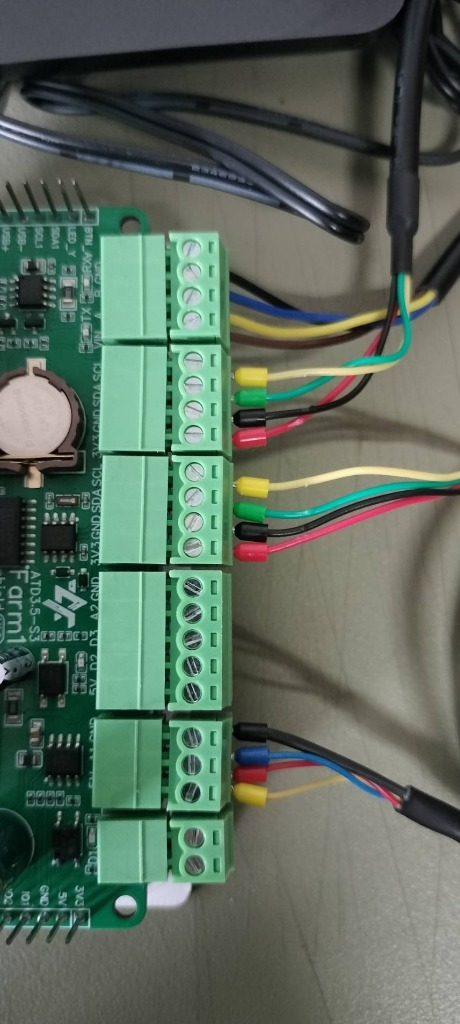
\includegraphics[width=0.55\textwidth]{figures/terminal_wiring.jpg}
    \caption{ลักษณะการต่อสายสัญญาณเซนเซอร์เข้ากับเทอร์มินัลบล็อกบนบอร์ด ATD3.5-S3 Farm1 Shield}
    \label{fig:terminal_wiring}
\end{figure}

\section{การจัดสรรขาสัญญาณไมโครคอนโทรลเลอร์ (Pin Assignment Configuration)}

เพื่อให้ระบบสามารถทำงานร่วมกับบอร์ด Farm1 Shield ได้อย่างเสถียรและป้องกันความขัดแย้งของฮาร์ดแวร์ภายใน ขาสัญญาณทั้งหมดได้รับการกำหนดไว้ในไฟล์เฮดเดอร์ \texttt{PinConfigs.h} ดังนี้

\begin{pythonbox}[การนิยามขาสัญญาณฮาร์ดแวร์ในไฟล์ PinConfigs.h]
#ifndef PIN_CONFIGS_H
#define PIN_CONFIGS_H

// 1. IPS Display 3.5" Controller: ST7796 (SPI Bus)
#define LCD_MOSI_PIN    11
#define LCD_MISO_PIN    13
#define LCD_SCK_PIN     12
#define LCD_CS_PIN      10
#define LCD_DC_PIN      14
#define LCD_RST_PIN     -1
#define LCD_BL_PIN      38  // Hardware Backlight control pin (Active HIGH)

// 2. Shared I2C Sensor Bus (SHT45 & BH1750 Dome)
#define I2C_SDA_PIN     9   // I2C Serial Data (Yellow Wire)
#define I2C_SCL_PIN     8   // I2C Serial Clock (Green Wire)

// 3. Analog ADC Input (Surface Soil Stick)
#define SOIL_STICK_PIN  1   // ADC1 Channel 0 (Terminal A1 on Shield)

// 4. Industrial RS485 Modbus RTU Port (7-in-1 Soil Sensor)
#define RS485_RX_PIN    41  // Hardware UART RX Pin
#define RS485_TX_PIN    40  // Hardware UART TX Pin
#define RS485_BAUD      4800

// 5. Actuator Control Relays (Active LOW Opto-isolated)
#define RELAY_PUMP_PIN  18  // Main Irrigation Water Pump Relay
#define RELAY_MIST_PIN  17  // Evaporative Cooling Misting Valve Relay

#endif // PIN_CONFIGS_H
\end{pythonbox}

\section{การสื่อสารผ่านบัส I2C ร่วมสำหรับเซนเซอร์บรรยากาศและแสงสว่าง}

การตรวจวัดสภาวะบรรยากาศรอบแปลงปลูกใช้เซนเซอร์ความแม่นยำสูง 2 ชนิดที่สื่อสารผ่านโพรโทคอล I2C\index{I2C} (Inter-Integrated Circuit) ร่วมกันบนโครงสร้างบัสเดียวกัน ได้แก่

\subsection{เซนเซอร์อุณหภูมิและความชื้นสัมพัทธ์ในอากาศ SHT45}
เซนเซอร์ \textbf{SHT45}\index{SHT45} ผลิตโดยบริษัท Sensirion บรรจุอยู่ในปลอกกรองโลหะซินเตอร์ (Sintered Metal Filter) ที่สามารถกันละอองน้ำและฝุ่นละอองในโรงเรือนได้อย่างมีประสิทธิภาพ โดยมีแอดเดรสฮาร์ดแวร์ประจำอุปกรณ์คือ \texttt{0x44} มีความคลาดเคลื่อนในการวัดอุณหภูมิต่ำเพียง $\pm 0.1\ ^\circ\text{C}$ และความชื้นสัมพัทธ์ $\pm 1.5\ \%\text{RH}$

\subsection{เซนเซอร์ความเข้มแสงกันน้ำโดมตะวัน}
เซนเซอร์ \textbf{โดมตะวัน (Sun Dome Sensor)}\index{BH1750} ใช้ชิปตรวจวัดแสงดิจิทัล BH1750FVI ที่ครอบด้วยโดมกระจายแสงทรงกลมสีขาวขุ่นเพื่อปรับแก้ค่าความเข้มแสงให้เป็นไปตามกฎโคไซน์ของแลมเบิร์ต (Lambert's Cosine Law) สื่อสารผ่านบัส I2C ด้วยแอดเดรส \texttt{0x23} สามารถวัดความเข้มแสงได้ตั้งแต่ 1 ถึง 65,535 Lux นอกจากนี้ ระบบยังแปลงค่าความเข้มแสง Lux เป็นค่าความหนาแน่นฟลักซ์พลังงานรังสีดวงอาทิตย์ (Solar Radiation Flux Density) ในหน่วยวัตต์ต่อตารางเมตร ($\text{W/m}^2$) โดยอาศัยความสัมพันธ์เชิงฟิสิกส์ $R_{\text{solar}} = \text{Lux} \times 0.0079\ \text{W/m}^2$ ซึ่งมีความสำคัญอย่างยิ่งต่อการประเมินการสะสมความร้อนและการระเหยน้ำในโรงเรือน

\begin{figure}[htbp]
    \centering
    \begin{minipage}[b]{0.48\textwidth}
        \centering
        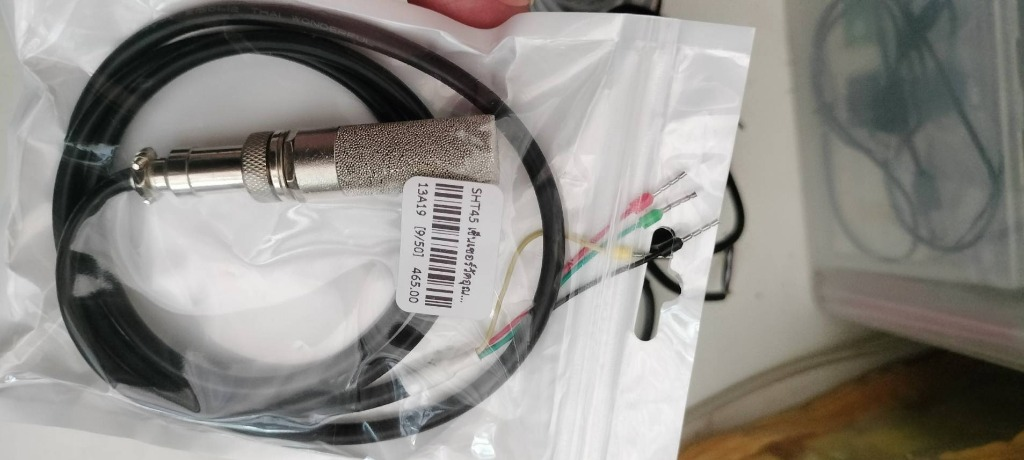
\includegraphics[height=5.0cm,width=\textwidth,keepaspectratio]{figures/sht45_sensor.jpg}
        \caption{เซนเซอร์ SHT45 วัดอุณหภูมิและความชื้นในปลอกกรองโลหะซินเตอร์}
        \label{fig:sht45_sensor}
    \end{minipage}
    \hfill
    \begin{minipage}[b]{0.48\textwidth}
        \centering
        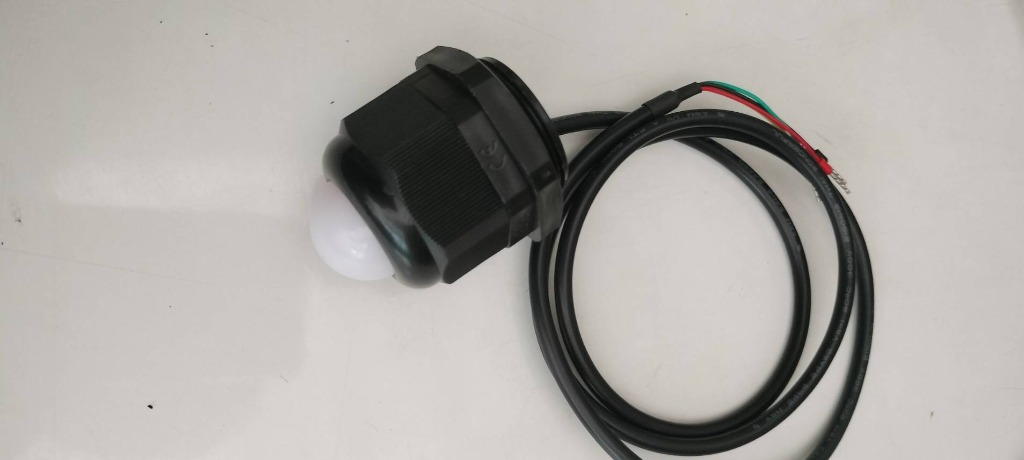
\includegraphics[height=5.0cm,width=\textwidth,keepaspectratio]{figures/light_dome.jpg}
        \caption{เซนเซอร์โดมตะวัน BH1750 วัดความเข้มแสงและรังสีอาทิตย์}
        \label{fig:light_dome}
    \end{minipage}
\end{figure}

เนื่องจากเซนเซอร์ SHT45 และโดมตะวัน BH1750 มีแอดเดรสบนบัส I2C ที่ไม่ซ้ำกัน จึงสามารถต่อสายสัญญาณร่วมกันบนเทอร์มินัลบล็อกเดียวกันได้โดยตรง จากการตรวจสอบด้วยระบบสแกนสัญญาณฮาร์ดแวร์ พบว่าการต่อสายจริงบนบอร์ด Farm1 Shield ได้กำหนดให้ \textbf{สายสีเหลืองเป็นสายข้อมูล SDA (GPIO9)} และ \textbf{สายสีเขียวเป็นสายสัญญาณนาฬิกา SCL (GPIO8)}

\section{การวัดความชื้นในดินผิวดินด้วยสัญญาณแอนะล็อกแบบคาปาซิทีฟ}

การตรวจวัดความชื้นบริเวณผิวดินระดับความลึก 0 ถึง 10 เซนติเมตร ใช้เซนเซอร์แท่งวัดความชื้น \textbf{Soil Stick เกษตรไทย IoT} ซึ่งทำงานด้วยหลักการเปลี่ยนแปลงค่าความจุไฟฟ้า (Capacitive Method) คลื่นความถี่สูง ซึ่งมีข้อได้เปรียบเหนือก้านวัดความต้านทานไฟฟ้า (Resistive Probes) ทั่วไป เนื่องจากไม่มีกระแสไฟฟ้าไหลผ่านเนื้อดินโดยตรง จึงไม่เกิดการกัดกร่อนจากปฏิกิริยาอิเล็กโทรลิซิส (Electrolysis Corrosion)

\begin{figure}[htbp]
    \centering
    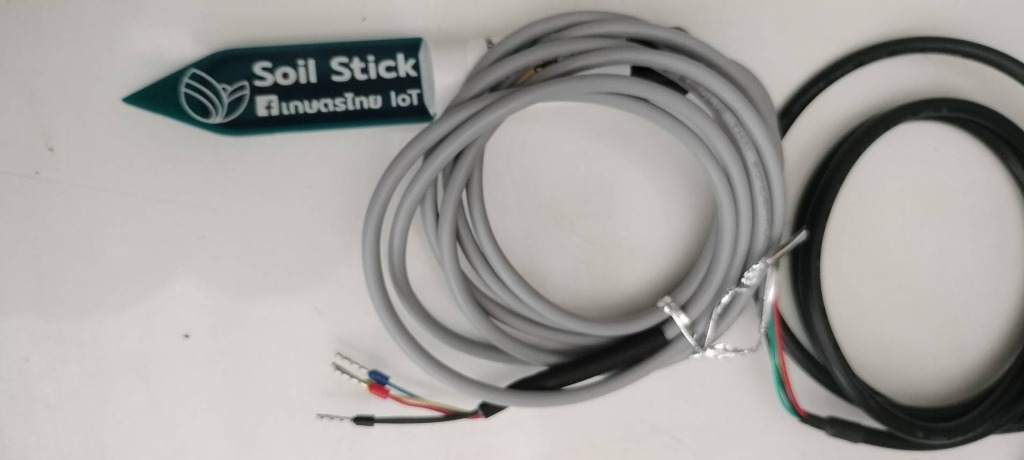
\includegraphics[height=5.2cm,width=0.65\textwidth,keepaspectratio]{figures/soil_stick.jpg}
    \caption{เซนเซอร์แท่งวัดความชื้นในดินผิวดิน Soil Stick เกษตรไทย IoT}
    \label{fig:soil_stick}
\end{figure}

สัญญาณแอนะล็อกจาก Soil Stick ถูกป้อนเข้าสู่ขาอะนาล็อก A1 (GPIO1) ของไมโครคอนโทรลเลอร์ ESP32-S3 ซึ่งถูกโปรแกรมให้ทำงานในโหมดตัวแปลงแอนะล็อกเป็นดิจิทัล (ADC) ความละเอียด 12 บิต (ช่วงค่า 0 ถึง 4,095) พร้อมตั้งค่าการลดทอนสัญญาณที่ $11\ \text{dB}$ เพื่อรองรับแรงดันไฟสูงสุด $3.1\ \text{V}$ ค่าความชื้นสัมพัทธ์ในดิน ($M_{\text{soil}}$) คำนวณผ่านสมการเชิงเส้นดังนี้

\begin{equation}
    M_{\text{soil}} = \left( \frac{\text{ADC}_{\text{air}} - \text{ADC}_{\text{raw}}}{\text{ADC}_{\text{air}} - \text{ADC}_{\text{water}}} \right) \times 100\%
    \label{eq:soil_moisture}
\end{equation}

โดยที่ $\text{ADC}_{\text{air}} = 2950$ แทนค่าสัญญาณดิบในอากาศแห้ง (ความชื้น 0\%) และ $\text{ADC}_{\text{water}} = 1450$ แทนค่าสัญญาณดิบเมื่อจุ่มในน้ำเปล่า (ความชื้น 100\%)

\section{การสื่อสารเชิงอุตสาหกรรม RS485 สำหรับคุณสมบัติดิน 7 พารามิเตอร์}

สำหรับการวิเคราะห์คุณสมบัติของดินในเขตรากพืชเชิงลึก (ความลึก 15 ถึง 30 เซนติเมตร) ระบบติดตั้งเซนเซอร์วัดดินอุตสาหกรรมแบบมัลติพารามิเตอร์รุ่น \textbf{SN-3002-TR-ECTHNPKPH-N01} ซึ่งมีเข็มวัดสแตนเลสสตีลทางการแพทย์ สามารถวัดค่าพร้อมกันได้ 7 พารามิเตอร์ ได้แก่ ความชื้นในดิน อุณหภูมิดิน สภาพนำไฟฟ้า (EC) กรด-ด่างดิน (pH) และปริมาณธาตุอาหารหลัก N-P-K

\begin{figure}[htbp]
    \centering
    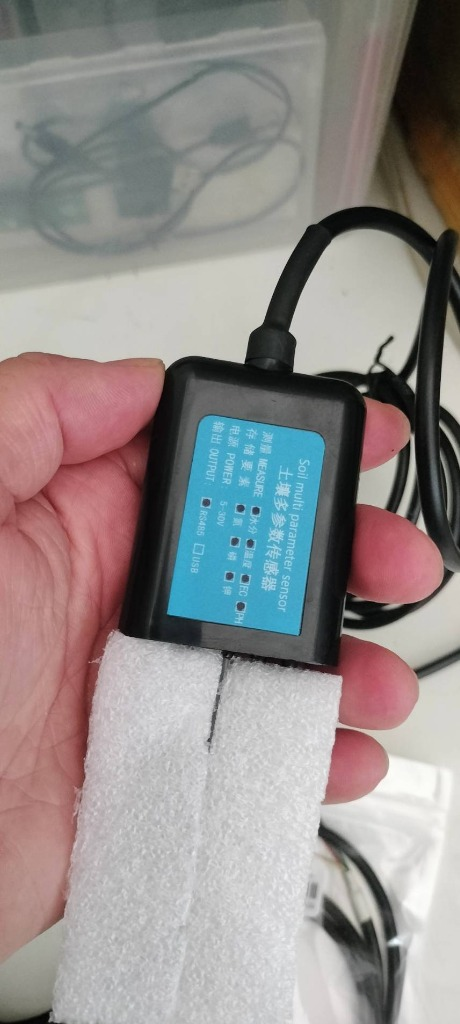
\includegraphics[height=5.5cm,width=0.60\textwidth,keepaspectratio]{figures/modbus_sensors.jpg}
    \caption{โพรบวัดคุณสมบัติดิน 7-in-1 Modbus RS485 สำหรับติดตั้งในเขตรากพืช}
    \label{fig:modbus_sensors}
\end{figure}

\begin{table}[htbp]
    \caption{การกำหนดค่าพารามิเตอร์และรีจิสเตอร์ Modbus RTU ของเซนเซอร์ดินรุ่น SN-3002}
    \label{tab:modbus_specs}
    \begin{tabularx}{\textwidth}{p{3.8cm}p{2.8cm}p{2.5cm}Y}
        \toprule
        \textbf{พารามิเตอร์} & \textbf{แอดเดรสรีจิสเตอร์} & \textbf{หน่วยวัด} & \textbf{ตัวคูณสเกลข้อมูล} \\
        \midrule
        ความชื้นในดิน (Moisture) & 0x0000 & \% & หารด้วย 10 (ทศนิยม 1 ตำแหน่ง) \\
        อุณหภูมิดิน (Temperature) & 0x0001 & $^\circ\text{C}$ & หารด้วย 10 (ทศนิยม 1 ตำแหน่ง) \\
        สภาพนำไฟฟ้า (EC) & 0x0002 & $\mu\text{S/cm}$ & จำนวนเต็มค่าตรง \\
        กรด-ด่างดิน (pH) & 0x0003 & pH & หารด้วย 10 หรือ 100 \\
        ไนโตรเจนที่ใช้ประโยชน์ (N) & 0x0004 & $\text{mg/kg}$ & จำนวนเต็มค่าตรง \\
        ฟอสฟอรัสที่ใช้ประโยชน์ (P) & 0x0005 & $\text{mg/kg}$ & จำนวนเต็มค่าตรง \\
        โพแทสเซียมที่ใช้ประโยชน์ (K) & 0x0006 & $\text{mg/kg}$ & จำนวนเต็มค่าตรง \\
        \bottomrule
    \end{tabularx}
\end{table}

ไมโครคอนโทรลเลอร์ ESP32-S3 ติดต่อกับเซนเซอร์ผ่านชิปแปลงสัญญาณ RS485 Transceiver โดยใช้พอร์ตสื่อสารอนุกรมฮาร์ดแวร์พอร์ตที่ 2 (HardwareSerial 2) กำหนดขา RX เป็น GPIO41 และขา TX เป็น GPIO40 ที่อัตราความเร็วรับส่งข้อมูล (Baud Rate) 4,800 bps

\subsection{การสร้างเฟรมคำสั่ง Modbus RTU และการคำนวณผลรวมตรวจสอบ CRC16}

เฟรมคำสั่งขออ่านข้อมูลแบบ Read Holding Registers (Function Code \texttt{0x03}) เพื่ออ่านข้อมูล 7 รีจิสเตอร์ต่อเนื่องกัน มีโครงสร้างขนาด 8 ไบต์ ประกอบด้วย
\begin{center}
\texttt{[0x01] [0x03] [0x00] [0x00] [0x00] [0x07] [0x04] [0x08]}
\end{center}
โดยที่สองไบต์สุดท้ายคือรหัสตรวจสอบความถูกต้อง CRC16 (Cyclic Redundancy Check) ซึ่งคำนวณผ่านพหุนาม $x^{16} + x^{15} + x^2 + 1$ (ค่าโพลีนอมิอัล \texttt{0xA001}) อัลกอริทึมการคำนวณในภาษา C++ ถูกอิมพลีเมนต์ดังนี้

\begin{pythonbox}[อัลกอริทึมการคำนวณ CRC16 Modbus ในภาษา C++]
uint16_t calculateModbusCRC(const uint8_t *buffer, size_t length) {
    uint16_t crc = 0xFFFF;
    for (size_t pos = 0; pos < length; pos++) {
        crc ^= (uint16_t)buffer[pos];
        for (int i = 8; i != 0; i--) {
            if ((crc & 0x0001) != 0) {
                crc >>= 1;
                crc ^= 0xA001;
            } else {
                crc >>= 1;
            }
        }
    }
    return crc;
}
\end{pythonbox}
